%% LaTeX file for Design representation
%% design.tex
%% 
%% Karlsruhe Institute of Technology
%% Version 1.0, 2018-12-13

%% Available page modes: oneside, twoside
%% Available languages: english, ngerman
%% Available modes: draft, final (see README)
\documentclass[oneside, english, final]{design}

\usepackage{graphicx}
\usepackage{caption}
\usepackage{pdfpages}
\usepackage[export]{adjustbox}

%usepackage{lipsum}


%% ---------------------------------
%% | Information about the thesis  |
%% ---------------------------------

%% Name of the author
\author{PSE Group}

%% Title (and possibly subtitle) of the thesis
\title{
Design}

%% Type of the thesis 
\thesistype{PSE}

%% The advisors are PhD Students or Postdocs
\advisor{M.Sc. Ankush Meshram}
%\begin{document}


%\end{document}
\thispagestyle{empty}

\settitle

%% --------------------------------
%% | Settings for word separation |
%% --------------------------------

%% Describe separation hints here.
%% For more details, see 
%% http://en.wikibooks.org/wiki/LaTeX/Text_Formatting#Hyphenation
\hyphenation{
% me-ta-mo-del
}

%% --------------------------------
%% | Bibliography                 |
%% --------------------------------

%% Use biber instead of BibTeX, see README
\usepackage[citestyle=numeric,style=numeric,backend=biber]{biblatex}
\usepackage{microtype}

\addtolength{\belowcaptionskip}{-10pt}
\setlength{\textfloatsep}{10pt plus 1.0pt minus 2.0pt}
%\addtolength{\abovecaptionskip}{-100pt}
\frenchspacing
%% ====================================
%% ====================================
%% ||                                ||
%% || Beginning of the main document ||
%% ||                                ||
%% ====================================
%% ====================================
\begin{document}
\nocite{*}

%% Set PDF metadata
\setpdf

%% Set the title
\maketitle

%% ----------------
%% |   Abstract   |
%% ----------------

%% The text is included from the following files:
%% - sections/abstract
\thispagestyle{empty}
\begin{abstract}
	\thispagestyle{empty}
\end{abstract}

%% -----------------
%% |   Main part   |
%% -----------------
\thispagestyle{empty}
\newpage
\thispagestyle{empty}
\tableofcontents
\cleardoublepage
\setcounter{page}{1}


\section{Design}\label{sec:intro}
\subsection{Front-End}

\subsubsection{Sequence Diagram}
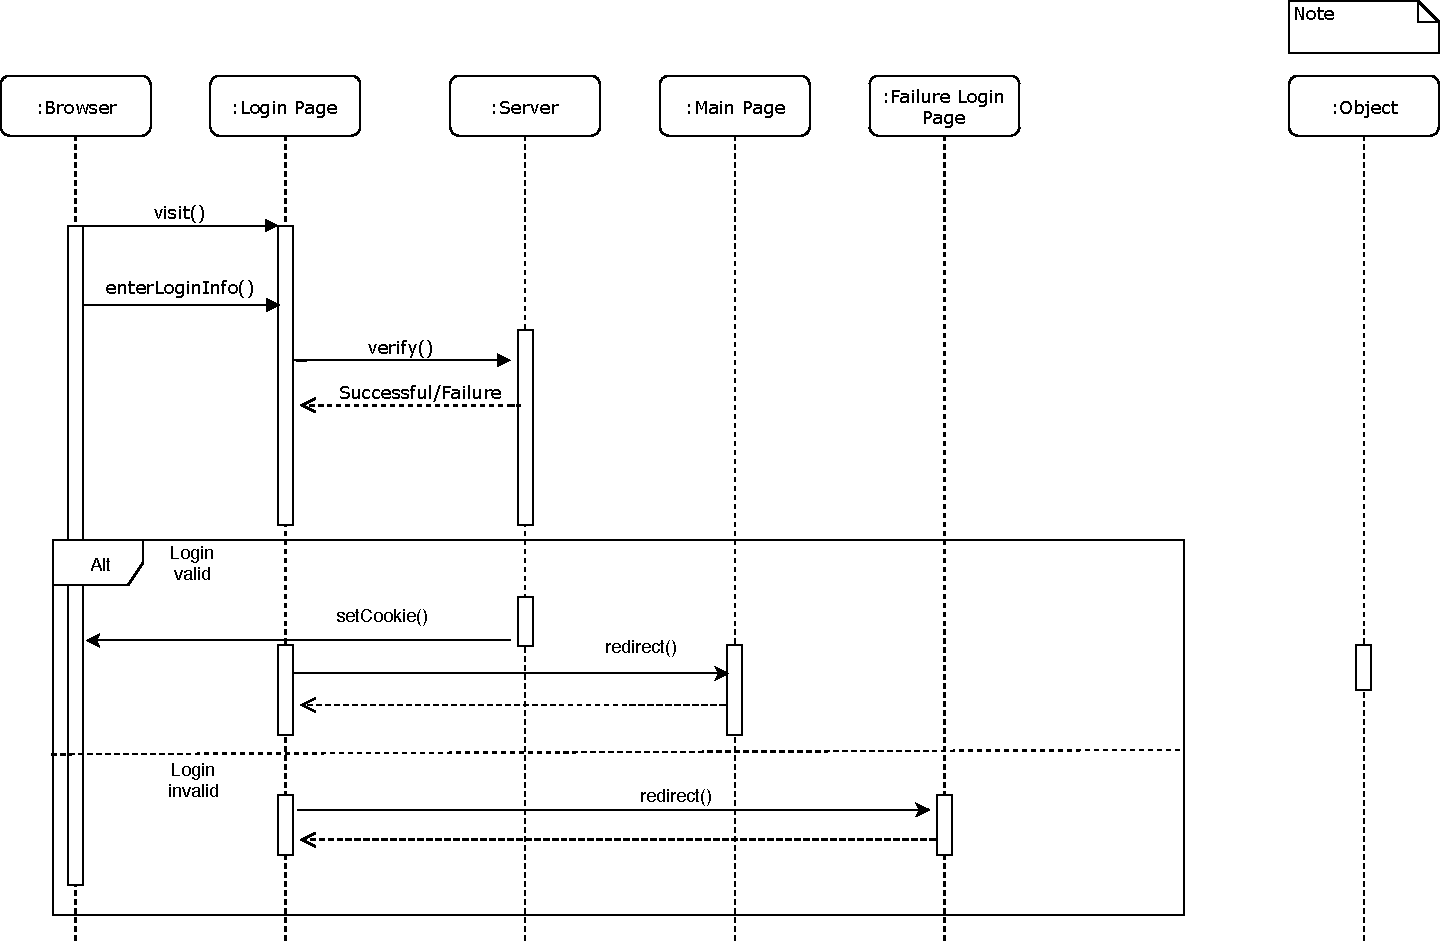
\includegraphics[max size={\textwidth}{\textheight}]{login1.pdf}
\newpage
The following diagram shows an alternative view of the login sequence:
\\
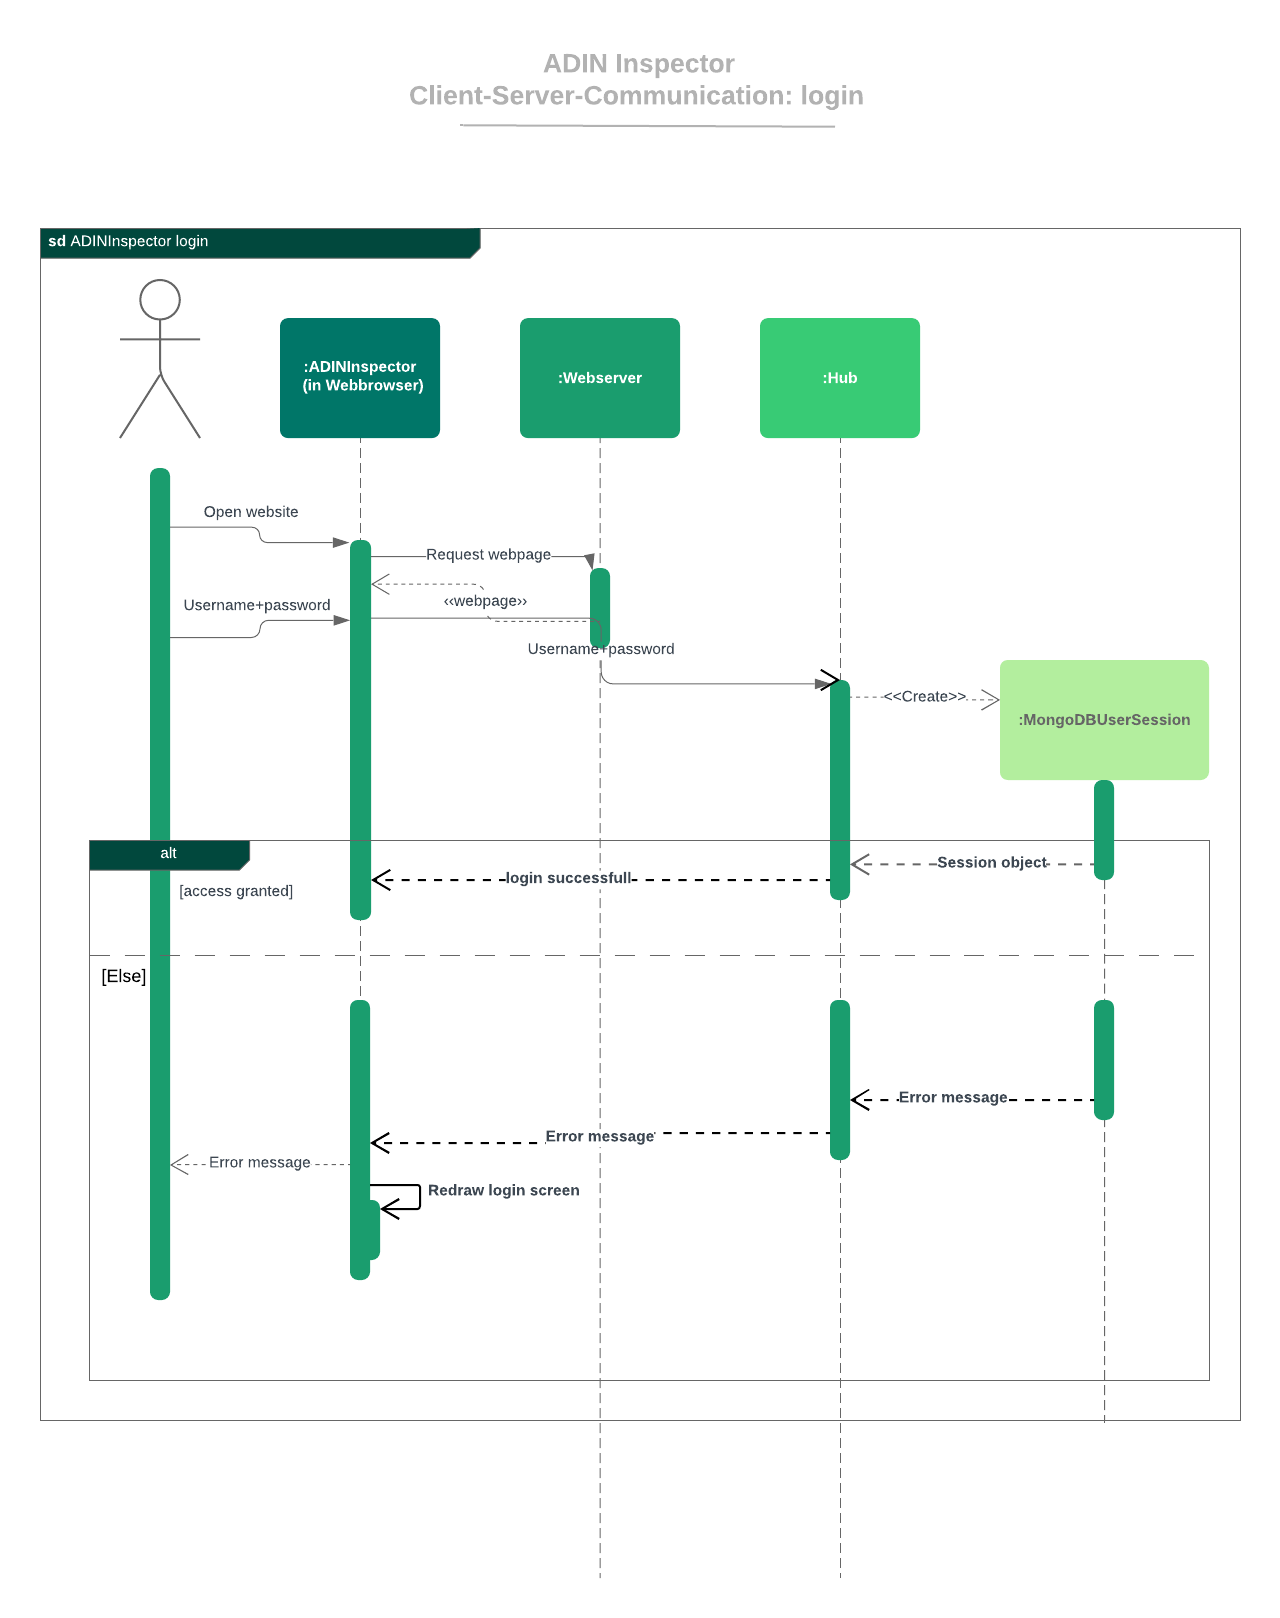
\includegraphics[max size={\textwidth}{\textheight}]{ADIN_Inspector_Client-Server-Communication-login.png}
\newpage
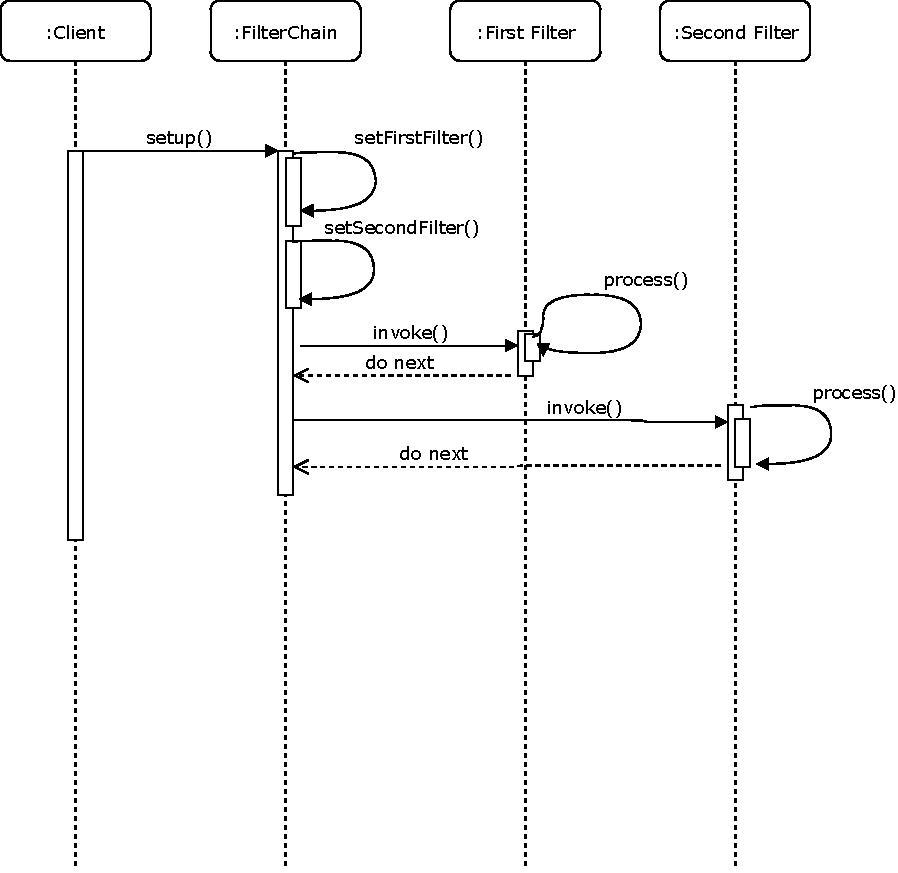
\includegraphics[max size={\textwidth}{\textheight}]{filterchain.pdf}
\newpage
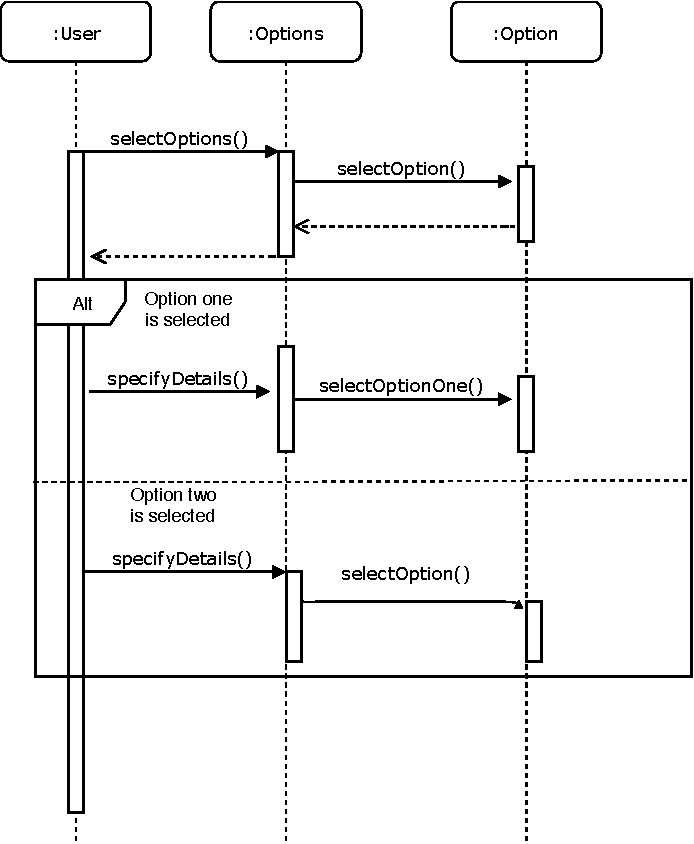
\includegraphics[max size={\textwidth}{\textheight}]{option.pdf}

\newpage
This diagram shows the control flow for handling a movement of the slider by the user.
% 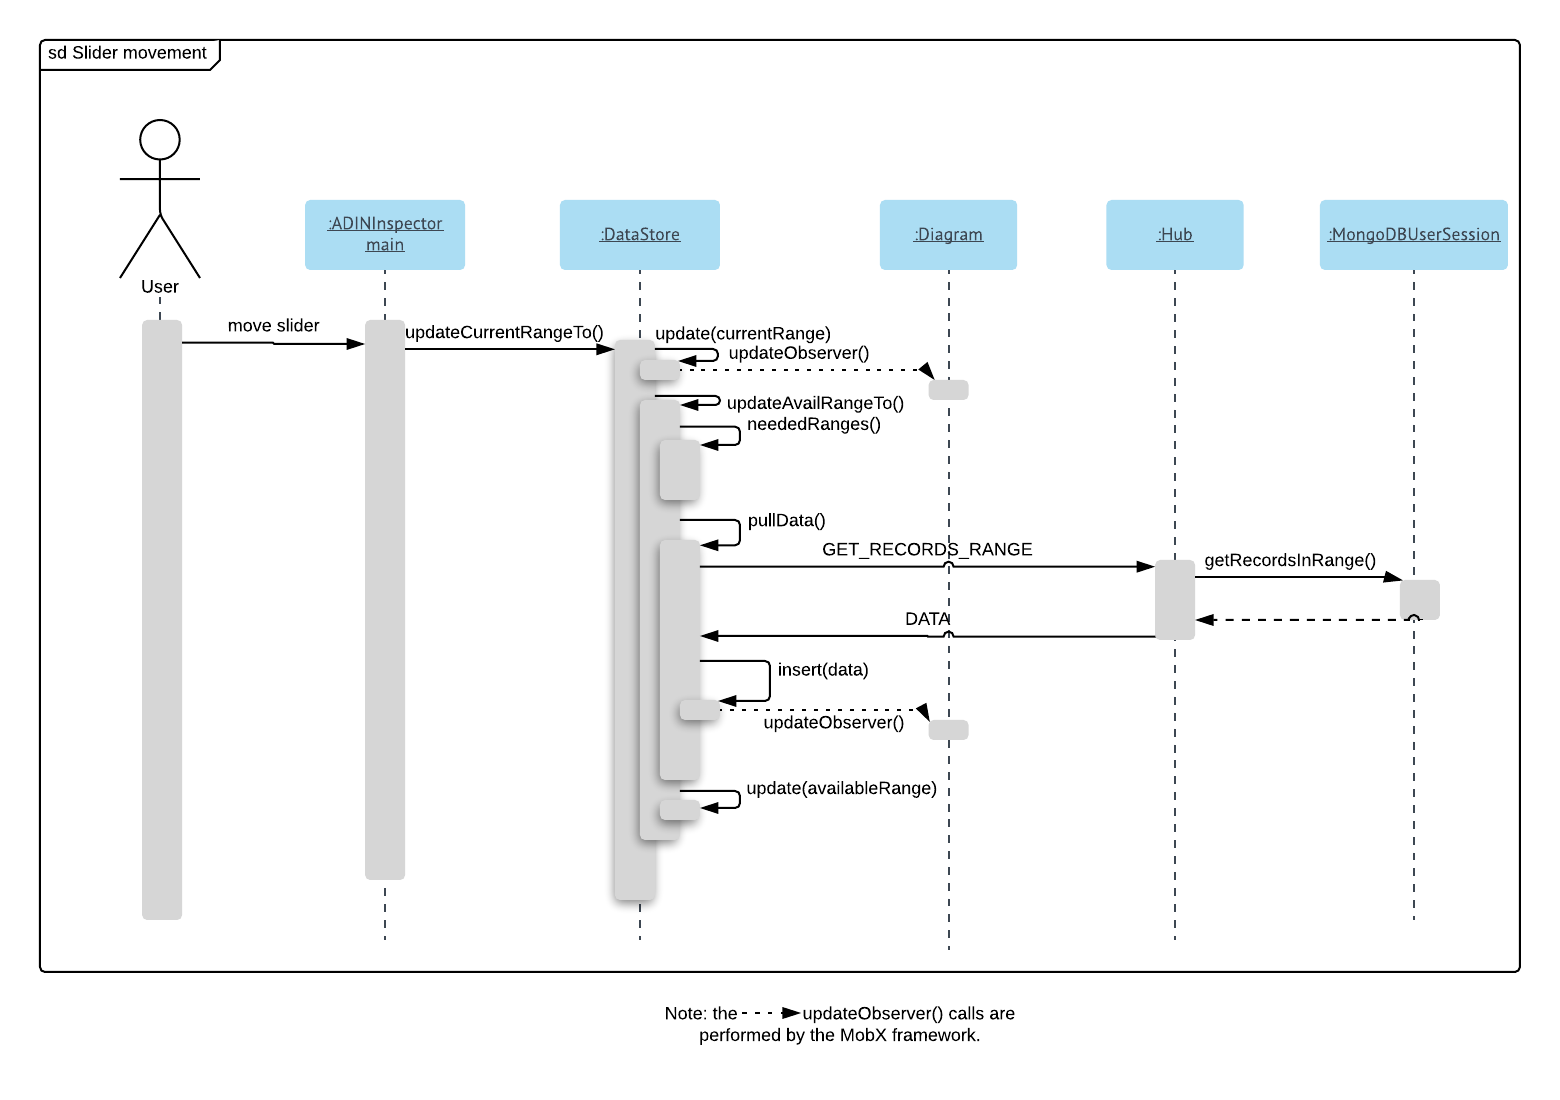
\includegraphics[max size={\textwidth}{\textheight}]{sd_frontend_comm-slider_movement.pdf}


\subsubsection{Activity Diagram}

\subsubsection{Class Diagram}

\begin{figure}
	\begin{adjustbox}
		{addcode={\begin{minipage}{\width}}
						{\caption{%
							This diagram shows an overview of GUI elements of the main application, when the user has successfully logged in.
						}
					\end{minipage}},rotate=90,center}
		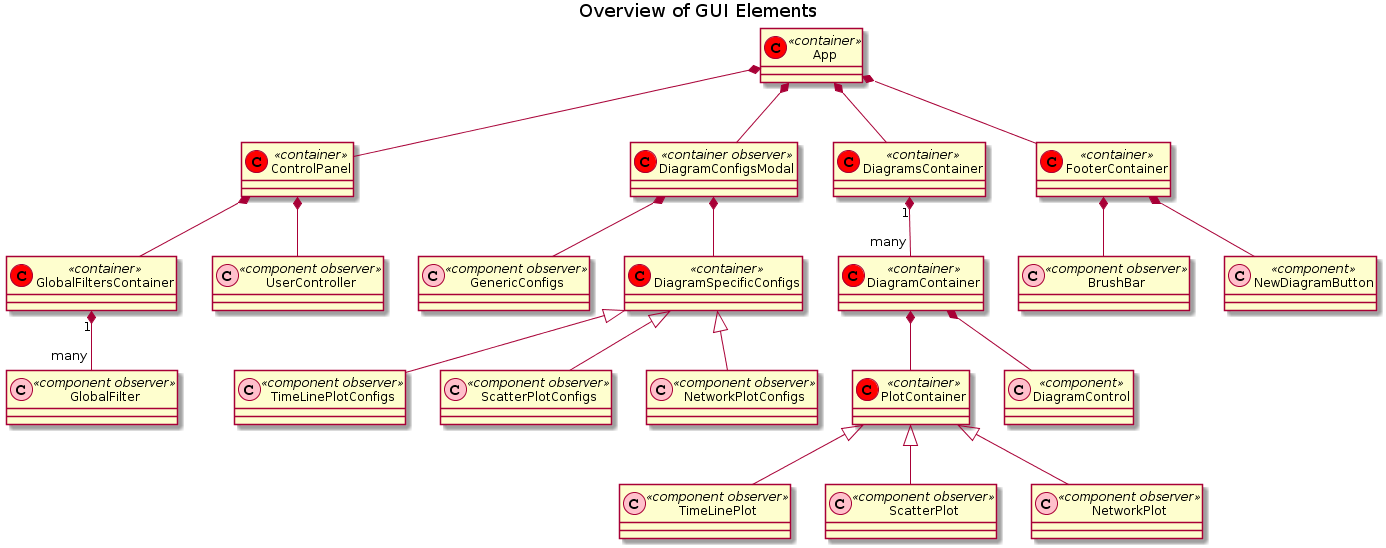
\includegraphics[max size={\textheight}{\textwidth}]{frontend/overview.png}%
	\end{adjustbox}
\end{figure}

\newpage



% 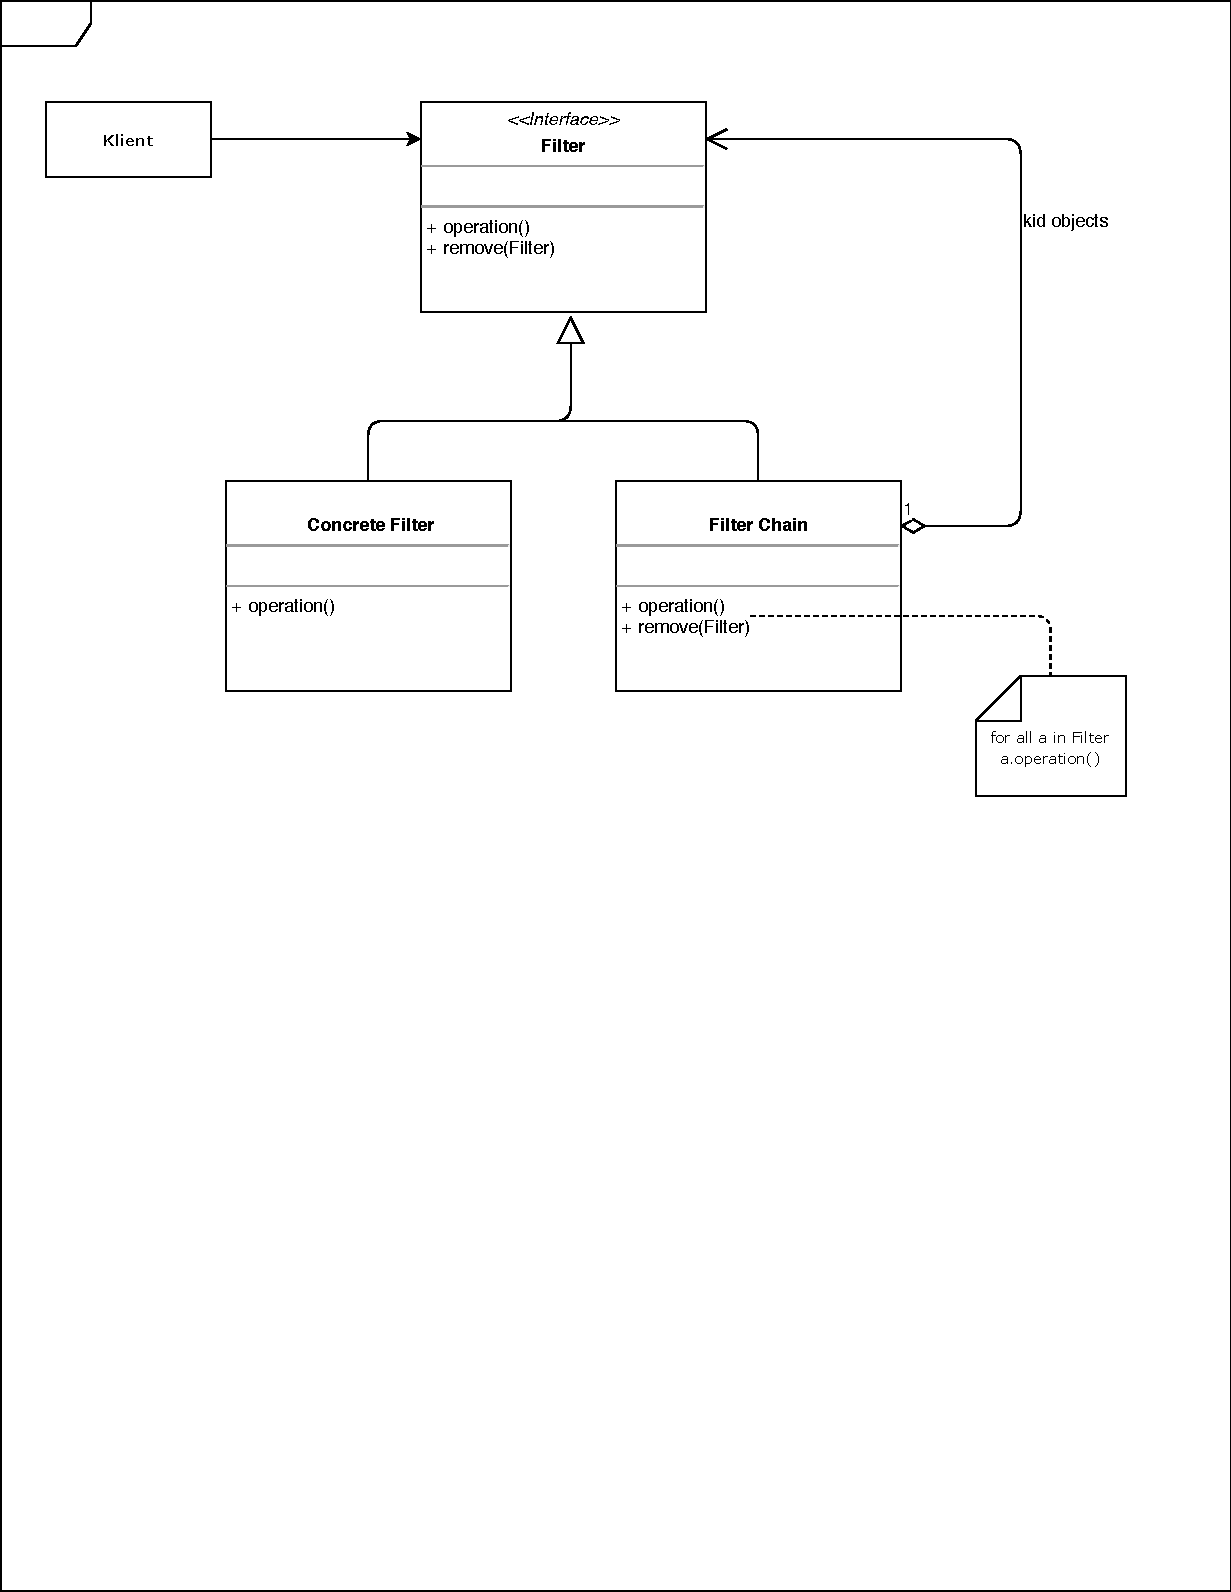
\includegraphics[max size={\textwidth}{\textheight}]{filterclassdiagram.pdf}
% \newpage
% 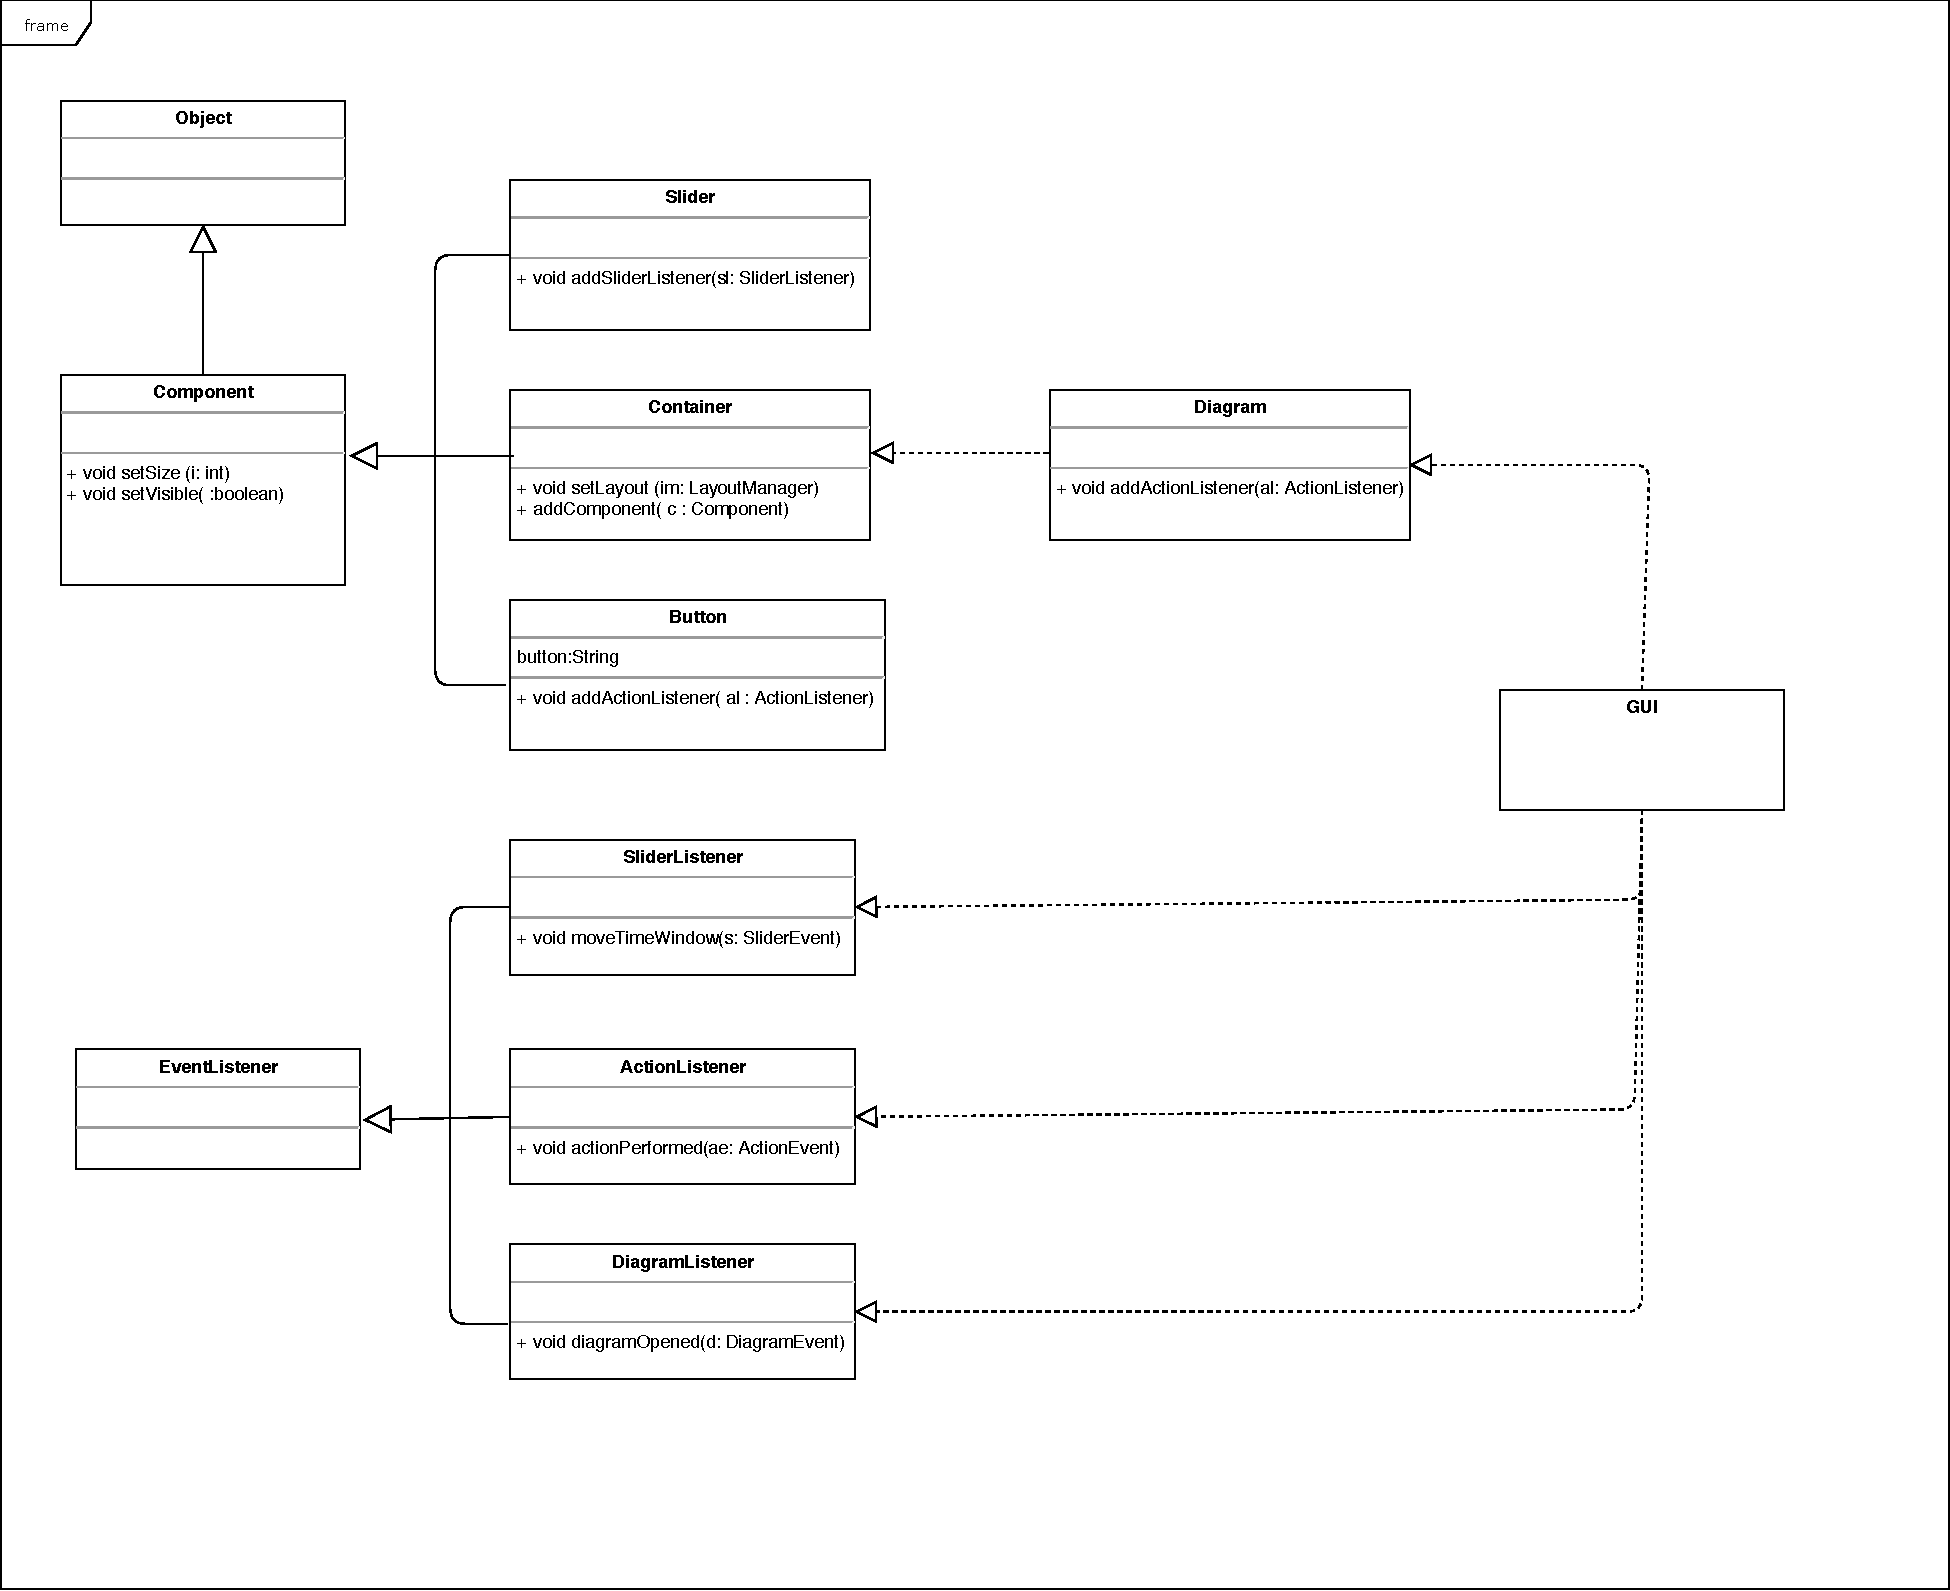
\includegraphics[max size={\textwidth}{\textheight}]{frame.pdf}
\newpage
\begin{figure}
	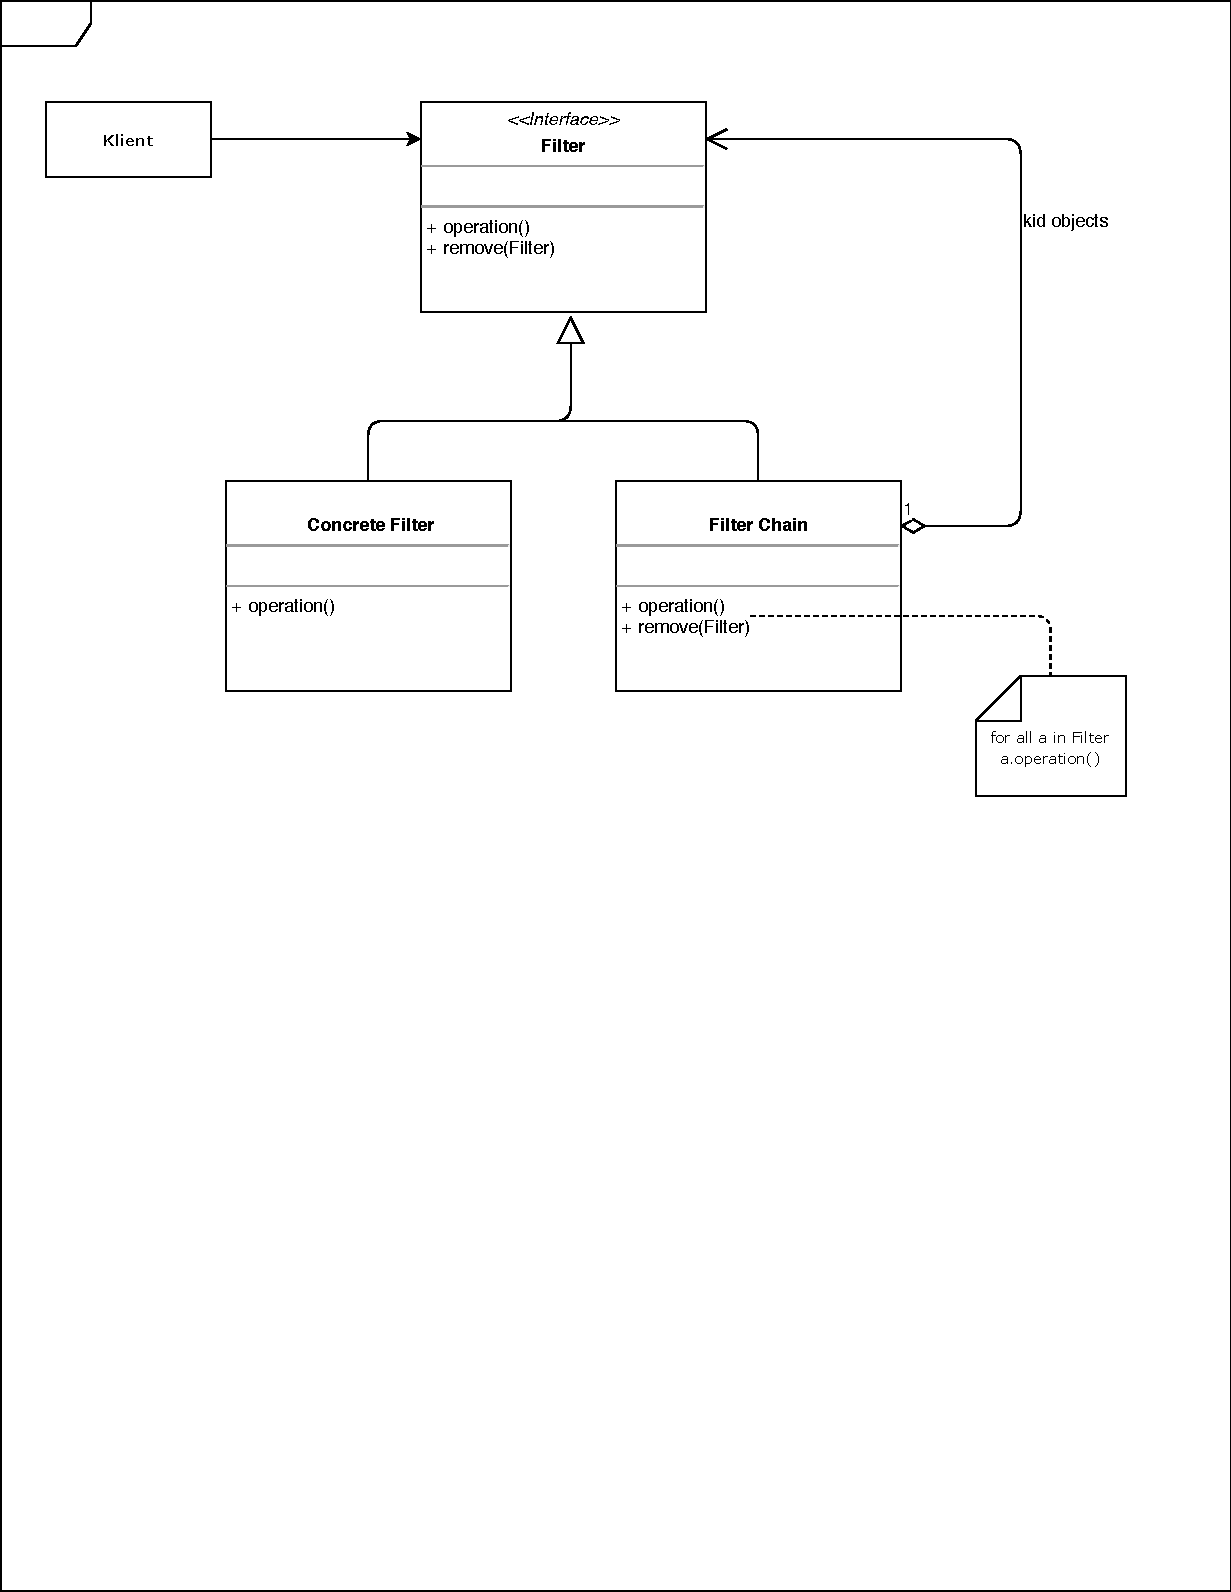
\includegraphics[max size={\textwidth}{\textheight}]{login2.pdf}
\end{figure}


\subsection{Client-server protocol}

Messages between client and server are exchanged as strings in JSON format.
\\
In the following list words in angle brackets ("<>") are placeholders.
\\

\subsubsection{Requests from client to server:}
\begin{itemize}
	\item{getAvailableCollections}
	      \\
	      syntax: \{"cmd": "GET\_AV\_COLL"\} \\
	      expected response: list of collections

	\item{getCollectionSize(collection)}
	      \\
	      syntax: \{"cmd": "GET\_COLL\_SIZE", "par": "<collection>"\} \\
	      where <collection> is the name of a collection\\
	      expected response: collection size

	\item{getCollection(collection)}
	      \\
	      syntax: \{"cmd": "GET\_COLL", "par": "<collection>"\} \\
	      expected response: data set

	\item{getRecordsInRange(collection, key, start, end)}
	      \\
	      syntax: \{"cmd": "GET\_RECORDS\_RANGE", "par": "<collection>", "key": "<keyvalue>", "start": "<startvalue>", "end:", "<endvalue>"\} \\
	      where <key> is the name of a key in the given collection and <startvalue> and <endvalue> are valid values for this key\\
	      expected response: data set

	\item{getRecordsInRangeSize(collection, key, start, end)}
	      \\
	      syntax: \{"cmd": "GET\_RECORDS\_RANGE\_SIZE", "par": "<collection>", "key": "<keyvalue>", "start": "<startvalue>", "end:", "<endvalue>"\} \\
	      expected response: collection size

\end{itemize}

\subsubsection{Messages from server to client:}
\begin{itemize}
	\item{list of collections}
	      \\
	      syntax: \{"cmd": "LIST\_COL", "par": ["<collection>"]\} \\
	      where <collection> is the name of a collection\\

	\item{collection size}
	      \\
	      syntax: \{"cmd": "COLL\_SIZE", "par": "<size>"\} \\
	      where <size> is the number of records in this collection\\
	\item{data set}
	      \\
	      syntax: \{"cmd": "DATA", "par": [<record>]\} \\
	      where each record is a JSON object
\end{itemize}

\subsection{Back-End}
This subsection deals with the back-end of the ADIN INSPECTOR. How the system deals with client http calls, and how kafka interacts with the system.
An overview of the system can be seen in \autoref{fig:class_back_end}

\subsubsection{Class Diagram}
Next we'll look at each class and method in detail

\begin{itemize}

	\item[•] Config properties file
	      \\The config file is stored alongside the built application .jar file and contains the path to the Kafka installation folder, the user name and password of a mongoDB account with the highest level of access and the name of the database.

	\item[•]Initializer
	      \\Methods:
	      \begin{itemize}
		      \item[-]main
		            \\ parameters: String of arguments from the console
		            \\ returns: void
		            \\ App entry point.
		            \\ We load the config.properties life and use the path provided to start the zookeper, kafka and mongodb services
	      \end{itemize}


	\item[•]MongoConsumer
	      \\The Mongo Consumer, as the name implies, consumes all messages from all topics in the Kafka messaging system. Once a message is found it is passed along to the Mongo Client for further processing.
	      \\Variables
	      \begin{itemize}
		      \item[-]clientMediator
		            \\Type : MongoClientMediator
		            \\ An instance of the Mongo Client Mediator, created with the credentials from the config file.
	      \end{itemize}
	      Methods
	      \begin{itemize}
		      \item[-]MongoConsumer constructor
		            \\parameters: user name and password of a mongoDB account with the highest level of access.
		            \\ Initializes the MongoClient variable and calls listenForRecords();
		      \item[-]getAllTopics
		            \\parameters: none
		            \\returns: an array of strings containing all the available kafka Topics.
		            \\Asks the kafka server service which topics exists.
		      \item[-]listenForRecords
		            \\parameters: none
		            \\returns: void
		            \\This Method first calls getAllTopics and uses the array of topics to poll the kafka server for new messages.
		            \\If new messages are found then the messages are passed to the Mongo Mediator for adding them to the Database.
		            \\If no new messages are found for a topic notify the Mongo Mediator that the collection tied to the topic is ready for pre-processing.
	      \end{itemize}


	\item[•]MongoClientMediator
	      This object serves as a nexus between the users who want to get data out of the database and the consumer and dataProcessor who want to add data into the database. This class encapsulates the mongo client from the mongo API.
	      \\Variables
	      \begin{itemize}
		      \item[-] client
		            \\type: MongoClient
		            \\ An instance of the Mongo Client from the official java API.
		      \item[-] dataProc
		            \\ A reference to the data processor class for this client.
	      \end{itemize}
	      Methods
	      \begin{itemize}
		      \item[-]MongoClientMediator constructor
		            \\parameters: Username and password
		            \\Initializes the client variable, throws an error if the user is not found.

		      \item[-]addRecordToCollection
		            \\parameters: String representation of a record in json format
		            \\String name of the collection it should be added to.
		            \\returns: void
		            \\Converts the json string into a java object, then to a bson document and uses the mongoAPI to insert it into the database.

		      \item[-]addRecordsToCollection
		            \\parameters: String Array of records to be added to a collection
		            \\String name of the collection it should be added to.
		            \\returns: void
		            \\for each oneof the members of the array call addRecordToCollection

		      \item[-]ProcessCollection
		            \\parameters: String, name of a collection
		            \\returns: void
		            \\signal the data processor to start the processing of a collection

		      \item[-]getCollection
		            \\parameters: String, name of a collection
		            \\returns: String array containing all entries of the collection

		      \item[-]getStartRecord
		            \\parameters: String, name of a collection
		            \\returns: the first entry of the collection as a String.

		      \item[-]getEndRecord
		            \\parameters: String, name of a collection
		            \\returns: the last entry of the collection as a String.

		      \item[-]getCollectionSize
		            \\parameters: String, name of a collection
		            \\returns: the number of entries in the collectoin as int

		      \item[-]getRecordsInRange
		            \\parameters: String, name of the collection to query
		            \\String, key of the parameter used for filtering
		            \\String start and end ranges for the filtering
		            \\returns: String array containing all entries of the collection within that range
		            \\this Method is very general to allow for flexibility.For example by letting the key be, SourceIPaddresses, or a timeStamp.

		      \item[-]getRecordsInRangeSize
		            \\parameters: String, name of the collection to query
		            \\String, key of the parameter used for filtering
		            \\String start and end ranges for the filtering
		            \\returns: number of elements matching the range as int


	      \end{itemize}

	\item[•]Record
	      \\Every message that comes from kafka and needs to be added to the database has it's own Record class that inherit from this one.
	      \\Every single class that inherits needs to be able to, using reflection, convert itself into a Bson Document where every variable is a key Value pair of the name of the variable and it's associated value.
	      \\Variables
	      \begin{itemize}
		      \item[-] id
		            \\type: String
	      \end{itemize}
	      Methods
	      \begin{itemize}
		      \item[-]getAsDocument()
		            \\parameters: none
		            \\returns: A Document, containing every variable of any class inheriting from this one.
		            \\This function checks for every variable, gets it's name and value as a string and adds it to the document that it eventually returns.
	      \end{itemize}

	\item[•]PacketRecord
	      \\Inheriting from Record, this class contains the variables that match the json string obtained from kafka.
	      \\Variables
	      \begin{itemize}
		      \item[-] id
		            \\type: String
		            \\this id is used for determining the ordering when saving to mongoDB, it's the offset of the message in the kafka messaging queue. inherited from Record
		      \item[-] client
		            \\type: String
		      \item[-] L2Protocol
		            \\type: String
		      \item[-] SourceMACAddress
		            \\type: String
		      \item[-] L4Protocol
		            \\type: String
		      \item[-] SourceIPAddress
		            \\type: String
		      \item[-] PacketSummary
		            \\type: String
		      \item[-] DestinationIPAddress
		            \\type: String
		      \item[-] Timestamp
		            \\type: String
		      \item[-] DestinationPort
		            \\type: String
		      \item[-] SourcePort
		            \\type: String
		      \item[-] DestinationMACAddress
		            \\type: String

	      \end{itemize}

	      Methods
	      \begin{itemize}
		      \item[-]getters / setters
		            \\parameters: variable
		            \\returns: variable type
		            \\Each variable has it's getters and setter methods.
	      \end{itemize}

	\item[•]AlarmRecord
	      \\Inheriting from Record, this class contains the variables that match the json string obtained from kafka.
	      \\Variables
	      \begin{itemize}
		      \item[-] id
		            \\type: String
		      \item[-] AlarmID
		            \\type: String
		      \item[-] AlarmType
		            \\type: String
		      \item[-] AlarmOccurrenceTime
		            \\type: String
		      \item[-] AlarmCategory
		            \\type: String
		      \item[-] AlarmScore
		            \\type: String
		      \item[-] AlarmDescription
		            \\type: String
		      \item[-] PacketSummary
		            \\type: String

	      \end{itemize}
	      Methods
	      \begin{itemize}
		      \item[-]getters / setters
		            \\parameters: variable
		            \\returns: variable type
		            \\Each variable has it's getters and setter methods.
	      \end{itemize}

	\item[•]MiscRecord
	      \\Inheriting from Record, this class is used by the data processor as an 'in-between' state before saving to the database. As well as an extension point for adding more types of records into the database programatically in the future.
	      \\Refer to the data processor class for further data on the key value pairs.
	      \\Variables
	      \begin{itemize}
		      \item[-] pairs
		            \\ A Map of strings to Objects to store any 1 to many relationships
	      \end{itemize}
	      Methods
	      \begin{itemize}
		      \item[-]getters / setters
		            \\parameters: none
		            \\returns: variable type
		            \\Each variable has it's getters and setter methods.
	      \end{itemize}

	\item[•]DataProcessor
	      \\This class is a mediator for each one of our data aggregators used for extraciton of features from the raw data stored in mongoDB.
	      \\ We might want to hve multiple data processors for chaining different aggregators together or to split up the work into mutliple threads. This is dependant on further performance testing.
	      \\Variables
	      \begin{itemize}
		      \item[-] client
		            \\ an instance of the associated mongoClient that requested the data aggregation
		      \item[-] aggregators
		            \\ A Arraylist containing all the aggregators to be applied on a collection.
	      \end{itemize}
	      Methods
	      \begin{itemize}
		      \item[-]getters / setters
		      \item[-]processData
		            \\parameters: variable
		            \\returns: variable type
	      \end{itemize}
	\item[•] IAggregator
	      \\This interface is the building block for every aggregator to be applied to data
	      \\Variables
	      Methods
	      \begin{itemize}
		      \item[-]processData
		            \\parameters: Records array of the records to be processed
	      \end{itemize}

	\item[•] FlowRatePerSecond
	      \\Implements IAggregator. This calculates, per port, the outgoing and ingoing connections.
	      A record processed by this aggregator is stored in a collection as follows:
	      \begin{verbatim} 
		  Name of collection: collectionName\_FlowratePerSec
		  structure of record as json:
		   {
		  "date" : \{" date" " Unix_Timestamp  } 
		  rounded down to the second this record points to.
		  Connections : [
		  { Port: "portNumer", "InOut" : " In/Out ", count : "Number" }
		  { Port: "portNumer", "InOut" : " In/Out ", count : "Number" }
		  ...
		  
		  ] This array has an entry per port if the port communicated that second. 
		  Precomputing this allows us to stream whenever the client needs the information 
		  for a specific node.
		}
	      \end{verbatim}
	      Methods
	      \begin{itemize}
		      \item[-]processData
		            \\parameters: Records array of the records to be processed
		            \\ specific imlpementation left to the classes implementing this interface
	      \end{itemize}

	\item[•] NumberOfConnectionsPerNodePerSecond
	      \\Implements IAggregator. This calculates the outgoing and ingoing connections.
	      A record processed by this aggregator is stored in a collection as follows:
	      \begin{verbatim} 
		  Name of collection: collectionName\_FlowratePerSec
		  structure of record as json:
		   {
		  "date" : \{" date" " Unix_Timestamp  } 
		  rounded down to the second this record points to.
		  Connections : [
		  { Port: "portNumer", count : "Number" }
		  { Port: "portNumer", count : "Number" }
		  ...
		  
		  ] This array has an entry per port if the port communicated that second. 
		  Precomputing this allows us to stream whenever the client needs the information 
		  for a specific node.
		}
	      \end{verbatim}
	      Methods
	      \begin{itemize}
		      \item[-]processData
		            \\parameters: Records array of the records to be processed
	      \end{itemize}

	\item[•]Hub
	      \\
	      This class implements the network handlers for the websocket connection to the client and access methods for a database connection.
	      \\Variables
	      \begin{itemize}
		      \item[-]requestHandler
		            \\Type : ClientProtocolHandler
		            \\ The strategy object we call for the actual parsing of the client requests.
	      \end{itemize}
	      \begin{itemize}
		      \item[-]database
		            \\Type : IUserSession
		            \\ The database we use during a user session.
	      \end{itemize}
	      Methods
	      \begin{itemize}
		      \item[-]handleOpen
		            \\parameters: Session session - the current session
		            \\returns: void
		            \\Event handler for the start of websocket connection.
		      \item[-]handleClose
		            \\parameters: Session session - the current session
		            \\returns: void
		            \\Event handler for closing a connection.

		      \item[-]handleMessage
		            \\parameters: String message - the message that we received from the client
		            \\Session session - the current session
		            \\returns: String - the response to be sent to the client
		            \\Event handler for receiving a message. The message is passed to the ClientProtocolHandler.

		      \item[-]handleError
		            \\parameters: Session session - the current session
		            \\Throwable t - the exception that occurred
		            \\returns: void
		            \\Event handler for errors/exceptions during communication.
	      \end{itemize}


	\item[•]IUserSession
	      \\An IUserSession object encapsulates a data base session.
	      On instantiation an IUserSession connects to a database using
	      the given user id and password and uses this connection for
	      all following data base access.
	      \\Methods
	      \begin{itemize}
		      \item[-]UserSession
		            \\parameters: String username - the user id to login with
		            \\String password - the password
		            \\returns: IUserSession
		            \\Factory method to instantiate a new UserSession and log in into the database using the given credentials.

		      \item[-]getAvailableCollections
		            \\parameters: -
		            \\returns: String array with collection names
		            \\Returns an array with the names of the collections available to the current user.

		      \item[-]getCollectionSize
		            \\parameters: String collection - the collection to query
		            \\returns: long - the number of records
		            \\Returns the number of records in the specified collection.

		      \item[-]getCollection
		            \\parameters: String - name of a collection
		            \\returns: String array containing all entries of the collection

		      \item[-]getRecordsInRange
		            \\parameters: String - name of the collection to query
		            \\String key - the parameter used for filtering
		            \\String start and end - range for the filtering
		            \\returns: String array containing all entries of the collection within the filter range
		            \\ Returns an array containing all records of this
		            collection for which the value of the
		            specified key is in the range [start, end).
		            The records will be in the same order as
		            they are in the collection.

		      \item[-]getRecordsInRangeSize
		            \\parameters: String - name of the collection to query
		            \\String key - the parameter used for filtering
		            \\String start and end - range for the filtering
		            \\returns: number of elements matching the range as int
		            \\Returns the number of records in the specified
		            collection for which the value of the specified
		            key is within the range [start, end).
	      \end{itemize}



	\item[•]MongoDBUserSession
	      \\Encapsulates a user session for a connection to a MongoDB database.
	      \\Methods
	      \begin{itemize}
		      \item[-]MongoDBUserSession constructor
		            \\parameters: -
		            \\Private constructor to create a new MongoDB session.

		      \item[-]UserSession
		            \\parameters: String username - the user id to login with
		            \\String password - the password
		            \\returns: a new MongoDBUserSession object
		            \\Factory method to instantiate a new MongoDBUserSession and log in into the database using the given credentials.

		      \item[-]getAvailableCollections
		            \\parameters: -
		            \\returns: String array with collection names
		            \\Returns an array with the names of the collections available to the current user.

		      \item[-]getCollectionSize
		            \\parameters: String collection - the collection to query
		            \\returns: long - the number of records
		            \\Returns the number of records in the specified collection.

		      \item[-]getCollection
		            \\parameters: String - name of a collection
		            \\returns: String array containing all entries of the collection

		      \item[-]getRecordsInRange
		            \\parameters: String - name of the collection to query
		            \\String key - the parameter used for filtering
		            \\String start and end - range for the filtering
		            \\returns: String array containing all entries of the collection within the filter range
		            \\ Returns an array containing all records of this
		            collection for which the value of the
		            specified key is in the range [start, end).
		            The records will be in the same order as
		            they are in the collection.

		      \item[-]getRecordsInRangeSize
		            \\parameters: String - name of the collection to query
		            \\String key - the parameter used for filtering
		            \\String start and end - range for the filtering
		            \\returns: number of elements matching the range as int
		            \\Returns the number of records in the specified
		            collection for which the value of the specified
		            key is within the range [start, end).

	      \end{itemize}

	      \newpage

	\item[•]ClientRequestHandler
	      \\This class handles client requests by parsing them, executing
	      the requested action and producing responses.
	      The requested actions are typically executed by calls to the database session object.
	      \\Methods
	      \begin{itemize}
		      \item[-]handleRequest
		            \\parameters: \\IUserSession  dbSession - the current database session
		            \\Session session - the current client session
		            \\String message - the client request to process
		            \\returns: String - the response to be sent to the client
		            \\Parse the message from the client, execute the requested action (typically a database query)  and construct the response message.
	      \end{itemize}


\end{itemize}

\begin{figure}
	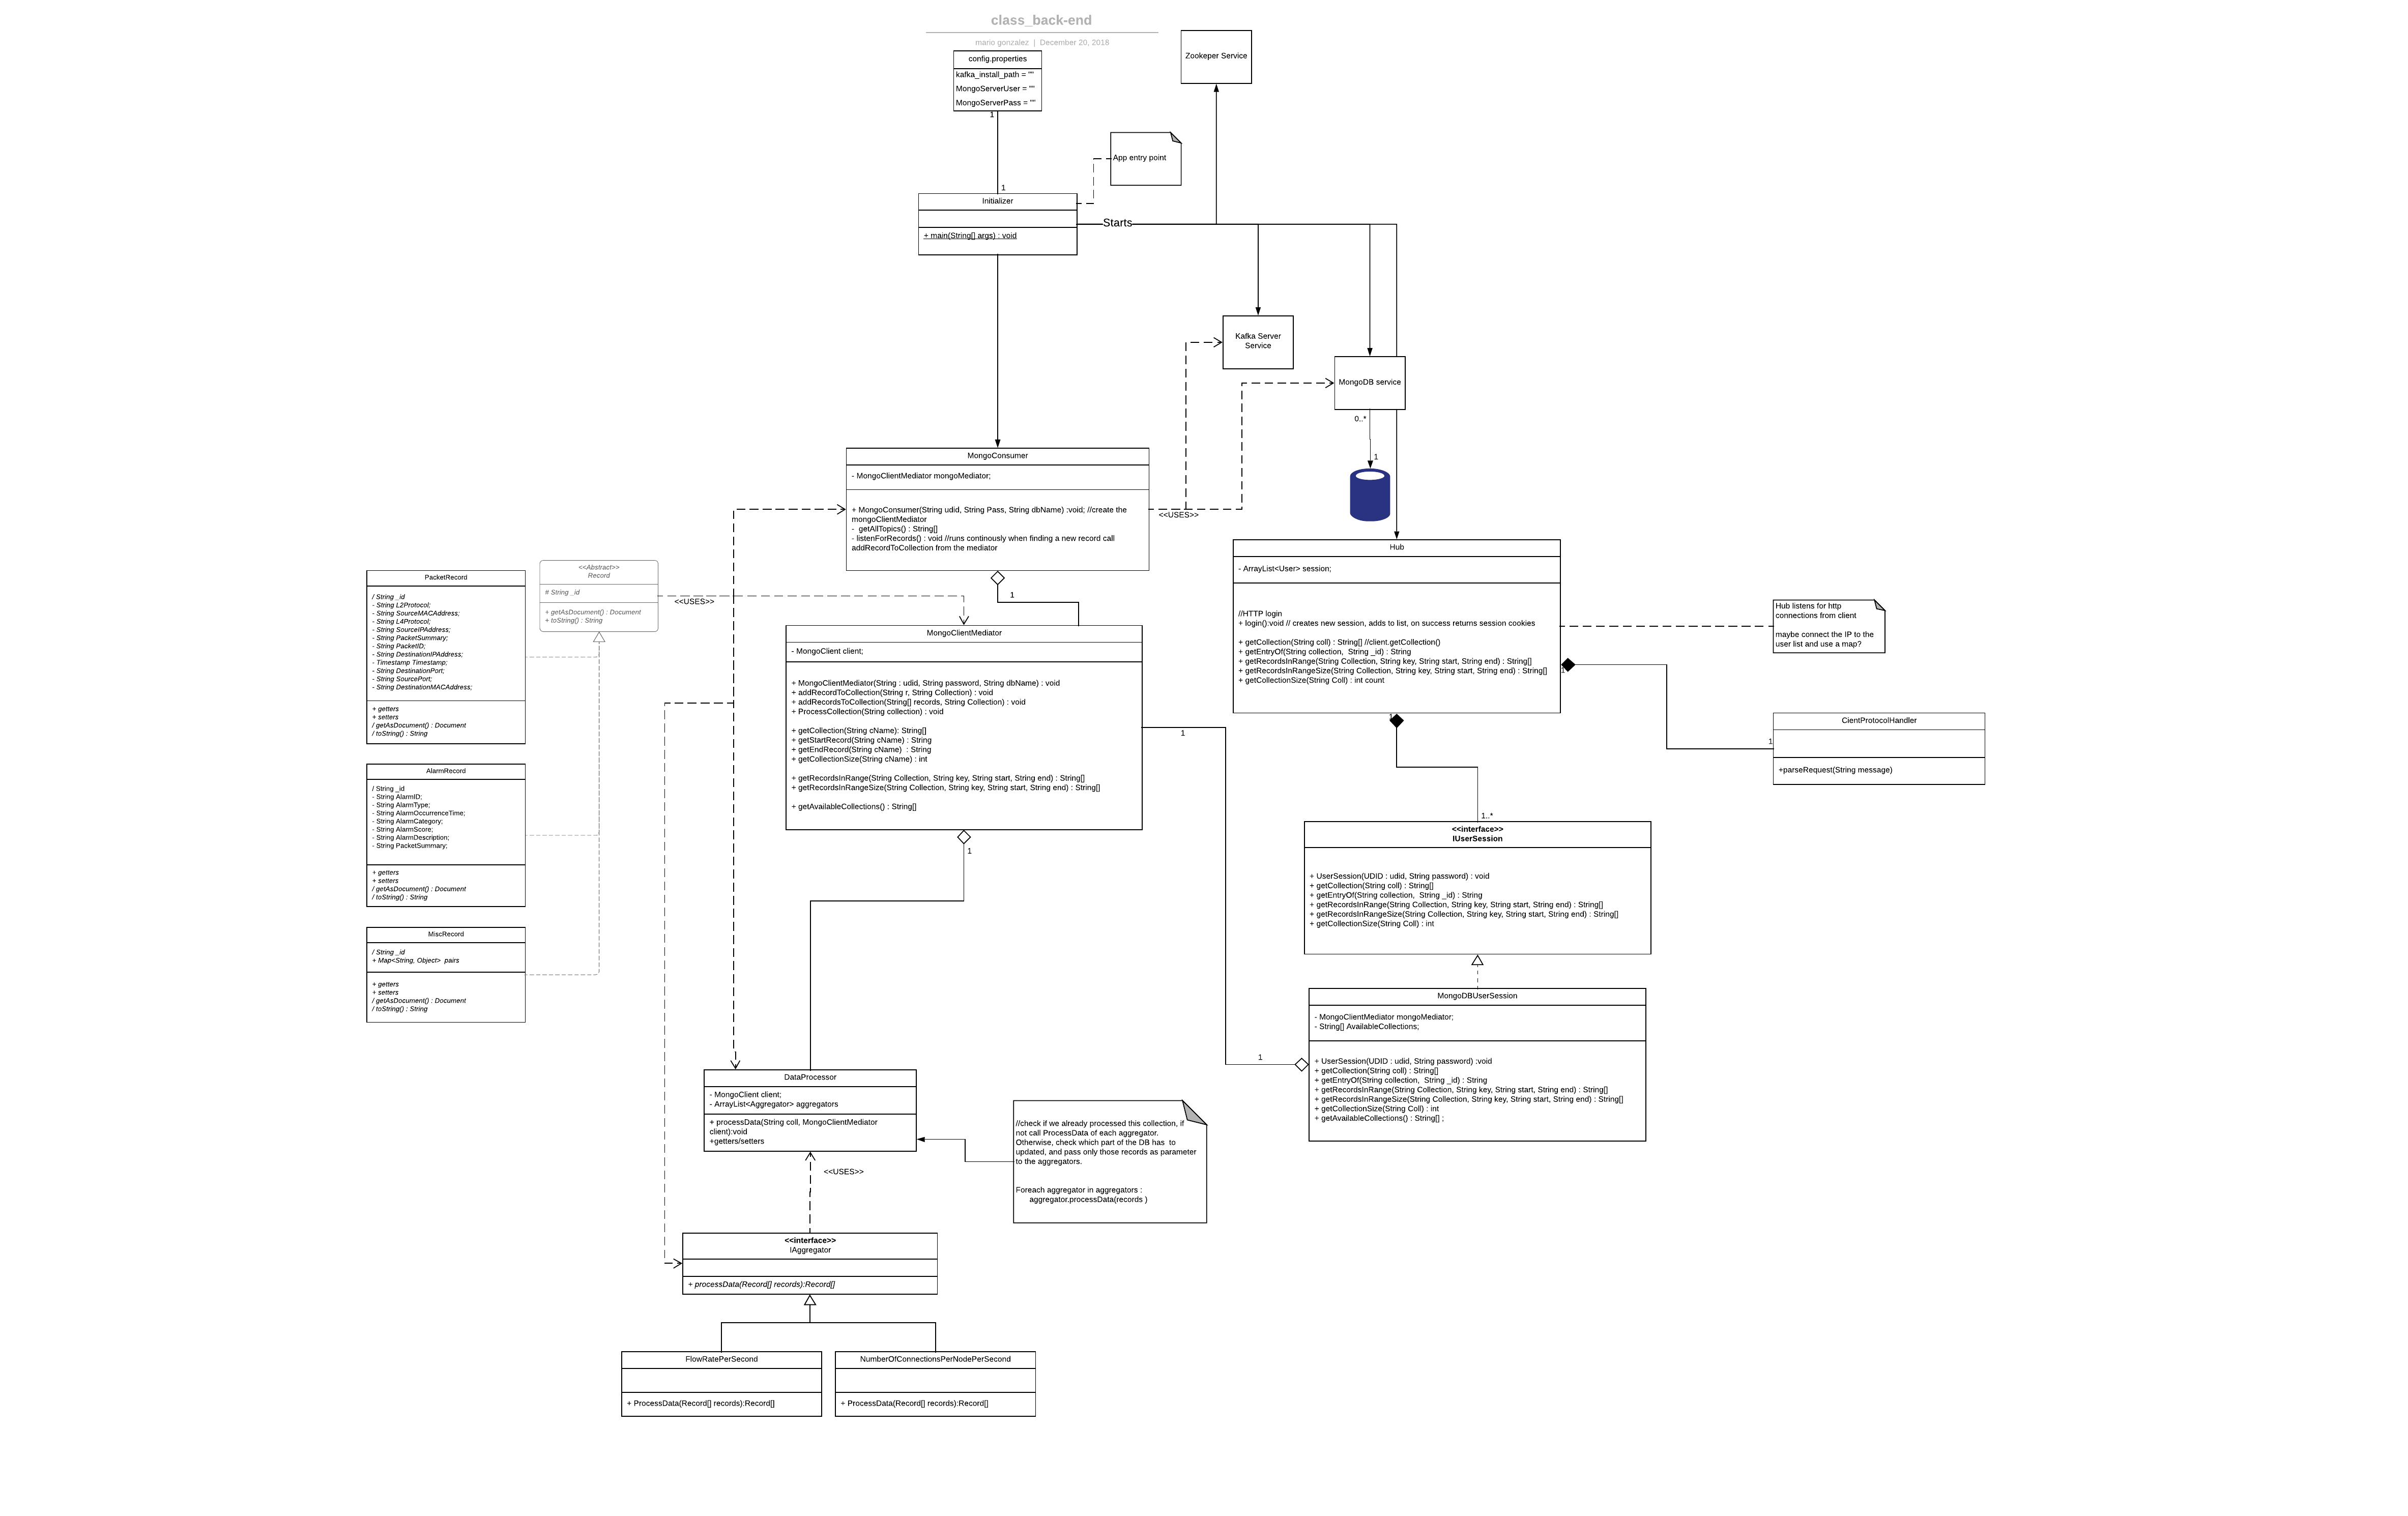
\includegraphics[angle=90,origin=c,max size={\textwidth}{\textheight}]{class_back-end.png}
	\caption{This is the class diagram for the whole back-end system}
	\label{fig:class_back_end}
\end{figure}
\newpage

\subsubsection{Sequence Diagram}
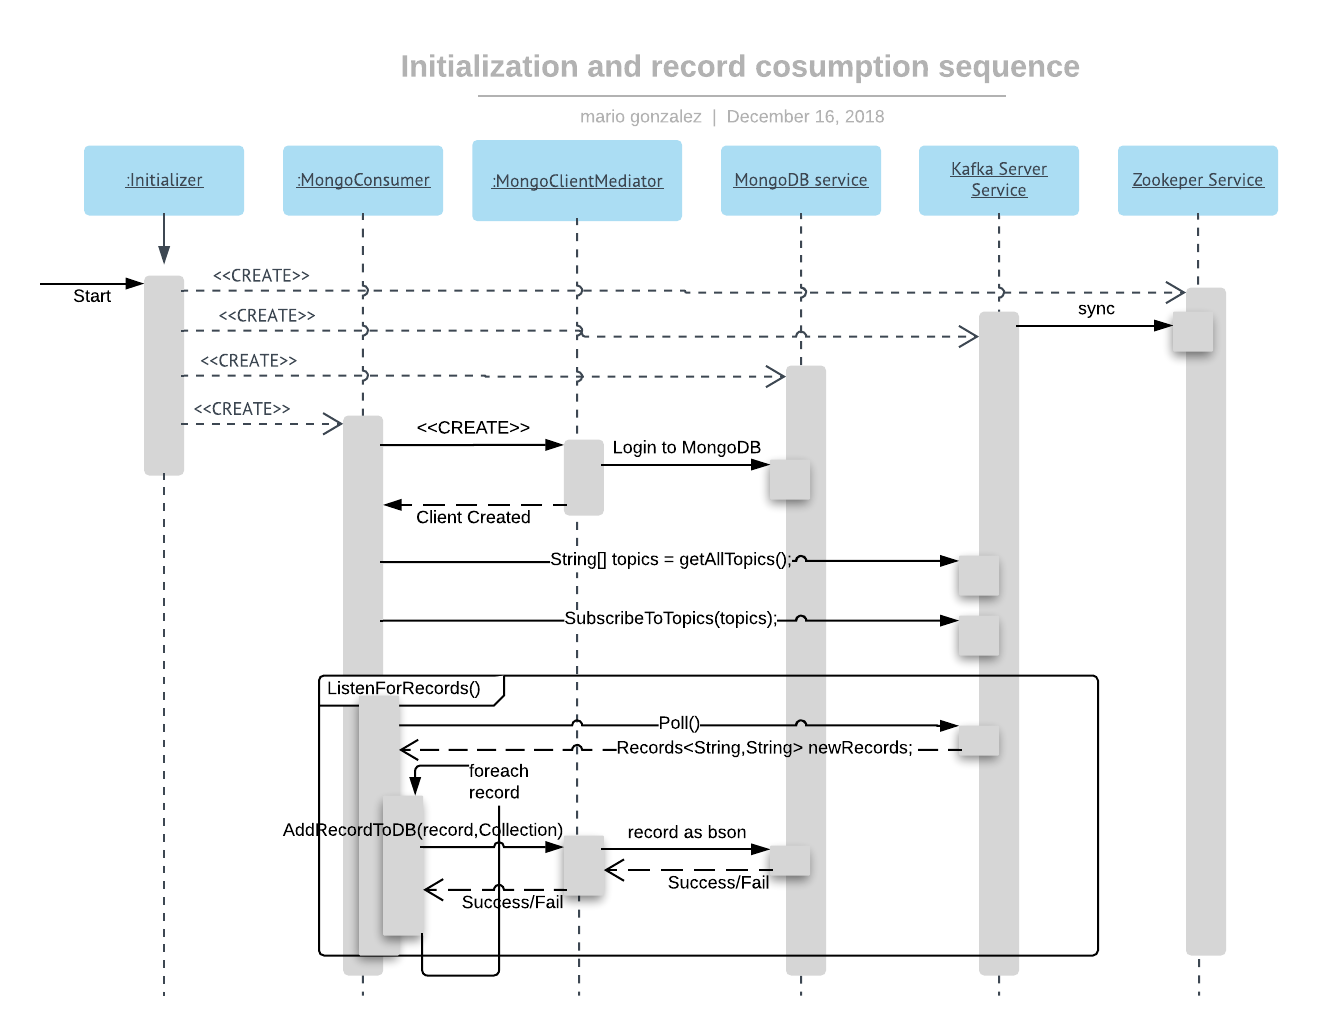
\includegraphics[max size={\textwidth}{\textheight}]{sequence_server_init.png}
\subsubsection{Activity Diagram}


\end{document}
